\tjformsection{二、\tjheadertext 方案介绍}\tjformsecnum{2}

\tjformsubsection{1．研究问题与研究内容}

本课题关注的核心问题是：单个开发者使用代码智能体完成开发任务时，如何将分散于对话、工具调用、代码变更与测试记录中的过程信息组织起来，使之可追溯、可核查，并在任务中断后支持上下文恢复。该问题包含三个相互关联的方面：一是采用何种信息模型统一表示异构记录，使任务、对话、变更、执行与测试之间能够建立稳定关联；二是依据哪些线索将上述记录归并到具体任务，并判定任务的起止边界；三是如何围绕代码变更组织证据、呈现任务进展，并在中断后恢复必要的上下文。三者分别对应表示、关联与恢复三个层面，评估则贯穿其中。研究方法上，拟采用文献分析、模型设计、原型实现与实证评估相结合的方式，先建立表示与关联方法，再通过原型检验其可用性。

围绕上述问题，本课题的研究内容主要包括五个方面。一是任务上下文的信息模型与统一事件表示，抽象开发任务、对话轮次、消息、工具调用、文件变更、测试运行、测试用例结果与检查点等实体及其关系，设计可扩展的事件模式，使不同来源的记录进入同一表示框架。二是上下文采集与关联，接入代码智能体的会话与工具调用、文件系统与 Git、测试报告，将编辑动作归一化为变更块，并利用时间邻近、显式引用与文件级位置映射等线索建立变更与对话之间的多对多关联。三是变更溯源与证据链，以变更块为单位记录触发来源、实施过程、修改前后快照、验证依据与后续演化，支持从代码到原因、从原因到代码的双向查询。四是交互界面与任务续接，设计任务中心、任务时间线与变更证据侧栏等视图，并在任务中断后生成任务快照，呈现已完成、未完成与待验证事项。五是大语言模型辅助与评估，在证据绑定约束下生成任务摘要与进展整理，并通过典型编程任务考察系统在代码理解、修改原因分析与任务衔接方面的作用。

\tjformsubsection{2．初步实施方案}

本课题的初步实施方案按“概念与模型—采集与关联—溯源与续接—评估”四个模块组织。四个模块对应研究推进的不同环节：概念与模型回答“表示什么”，采集与关联回答“如何获得并建立联系”，溯源与续接回答“如何查询与使用”，评估回答“方案是否有效”。四者并非软件工程的层次划分，而是相互约束的研究环节，其关系如图~\ref{fig:route} 所示。

\begin{figure}[H]
  \centering
  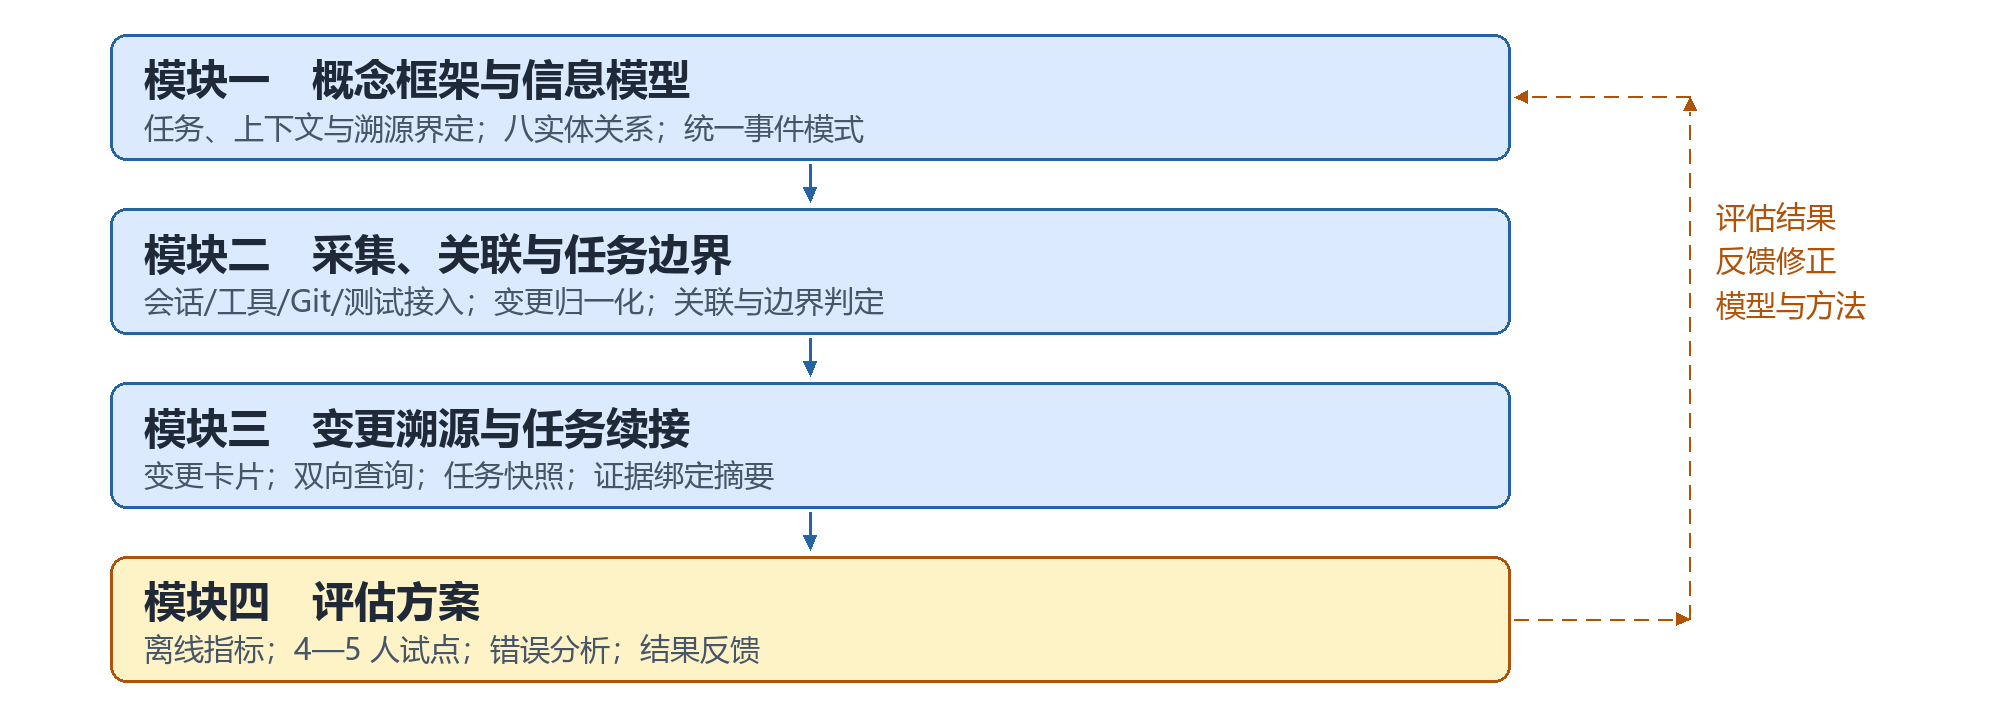
\includegraphics[width=\linewidth]{figures/fig1-route.png}
  \caption{研究技术路线}
  \label{fig:route}
\end{figure}

\tjformsubsub{（一）概念框架与信息模型}

本模块界定开发任务、任务上下文与变更溯源三个核心概念，并提出可计算的信息模型。开发任务指开发者发起的一次有明确目标的开发工作单元；任务上下文指与该任务相关的对话、变更、执行、测试、决策与未完成事项的集合；变更溯源指从一段代码变更出发，追溯其触发来源、实施过程、验证依据与后续演化的证据链。在此基础上，将任务上下文刻画为以任务为根的有向异构图：节点包括任务、对话轮次、消息、工具调用、文件变更、测试运行、测试用例结果与检查点，边包括包含、触发、产出、验证、演化与快照等关系。该模型与 PROV-O[32] 的基本思想一致，但针对智能体事件流增加了任务边界、变更块与验证依据等约束。事件采用统一的 JSON 结构表示，字段涵盖标识、类型、时间、主体、来源、载荷与关联；模型需满足变更标识稳定、消息与变更多对多、测试结果双向指向等基本约束。上述概念与模型为后续采集、关联与查询提供共同语言，其具体表结构与索引方式将在原型实现阶段细化。

\begin{figure}[H]
  \centering
  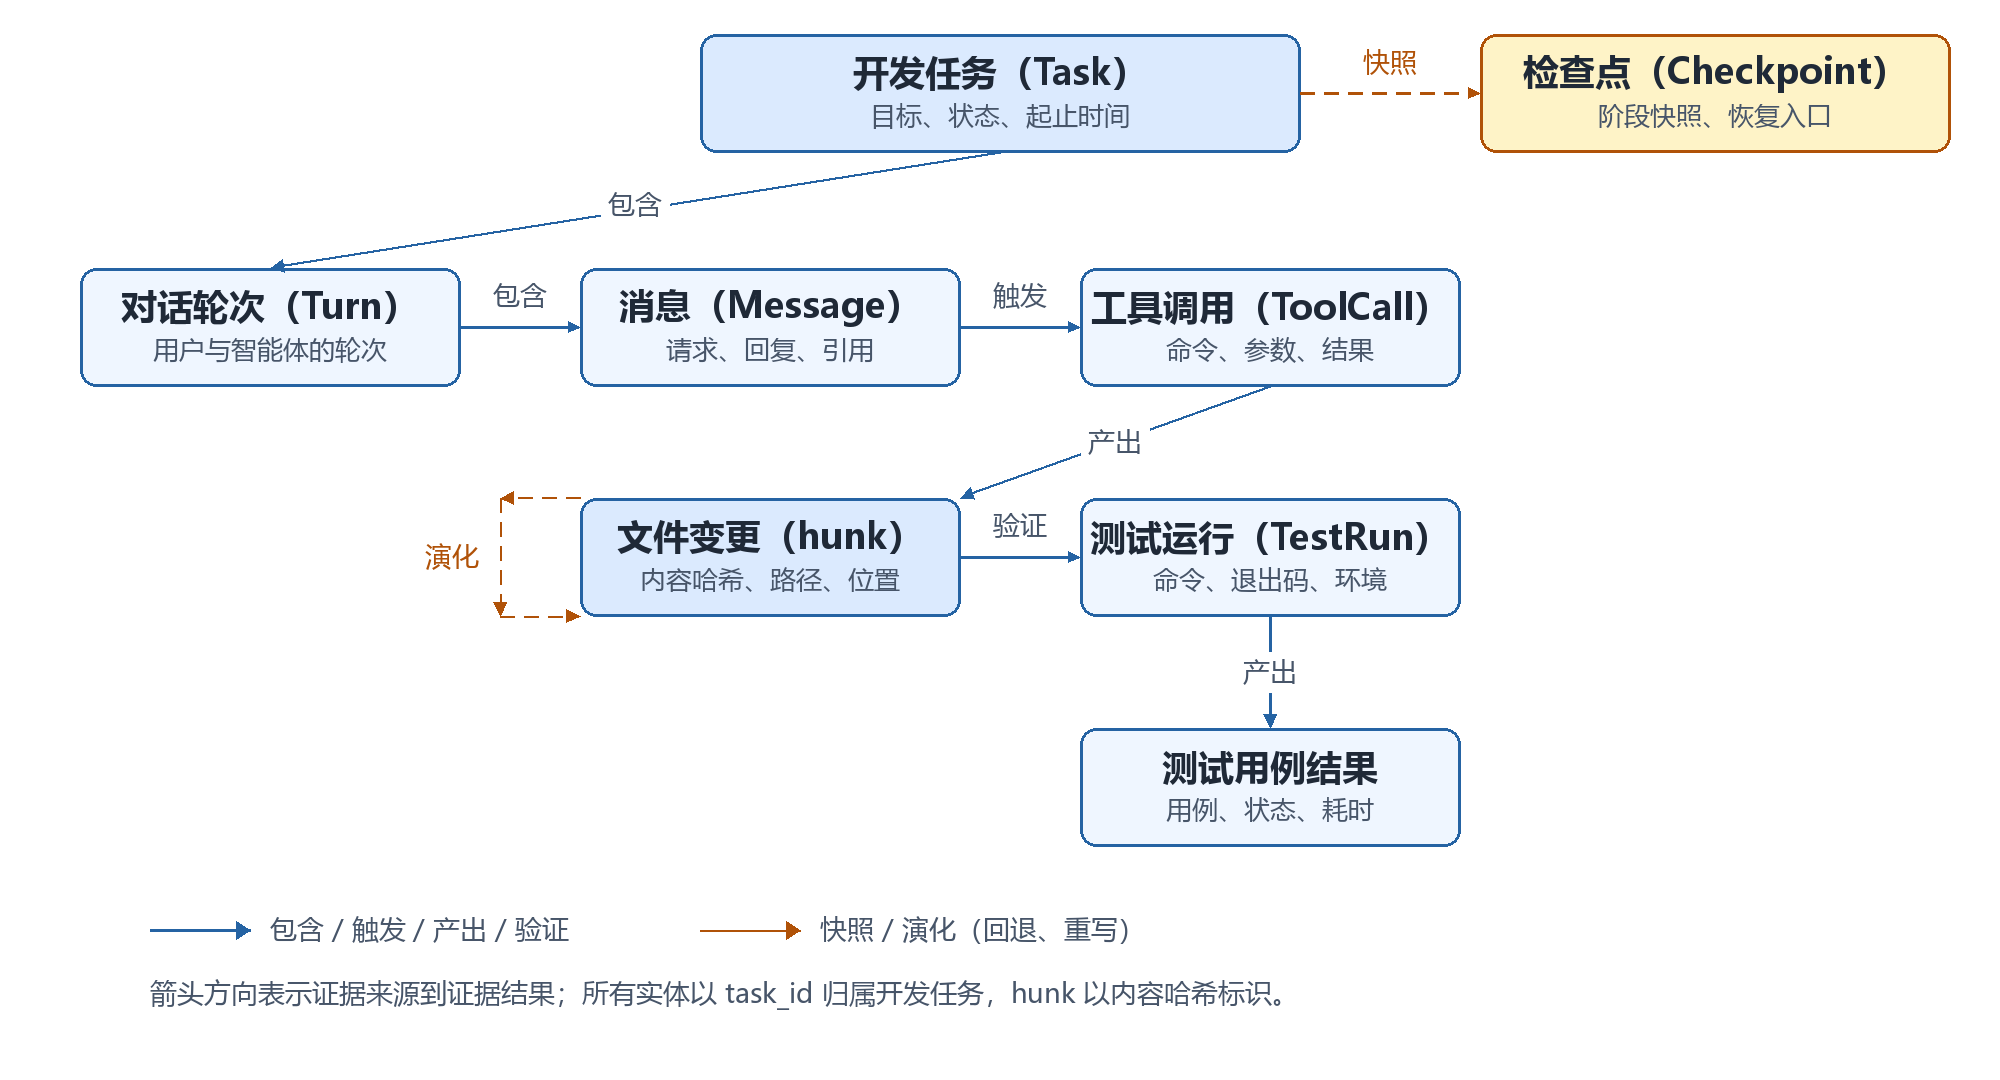
\includegraphics[width=\linewidth]{figures/fig2-model.png}
  \caption{任务上下文的信息模型}
  \label{fig:model}
\end{figure}

\tjformsubsub{（二）上下文采集、关联与任务边界}

本模块研究如何从真实开发过程中获得上述实体，并建立它们之间的关联。采集对象包括代码智能体的会话与工具调用、文件系统与 Git 变更、测试运行与结果；接入方式以 Claude Code 的官方钩子与 stream-json 为主，本地日志与 Git 作为补充。由于不同工具的编辑动作形式不一，需要将“旧串→新串”、补丁、整文件写入等统一归一化为变更块；语法感知的符号定位可借助 tree-sitter[41] 一类解析器完成。关联层面，拟综合利用时间邻近、显式引用（路径、符号、行号、命令、测试名）与文件级位置映射三类线索，为每条消息与每个变更块计算关联强度，并保留多对多关系。任务边界判定则依据空闲时长、显式指令、目标切换与提交动作等特征，采用可解释的规则打分，以便向开发者说明判定依据。该模块的重点不在于追求单点最优，而在于形成一套可复现、可解释的关联流程，其参数与阈值将在小规模验证集上调整并报告敏感性。

\tjformsubsub{（三）变更溯源与任务续接}

本模块将前两个模块的表示与关联转化为开发者可查询、可使用的证据链。对每个变更块生成变更卡片，记录触发消息、相关工具调用、修改前后快照、验证测试与后续演化；查询支持从代码到原因、从原因到代码两个方向。任务续接以任务快照为核心：快照由任务上下文图生成，将事项分为已完成、未完成与待验证三类，并附带指向证据的链接，使开发者能够从摘要直接跳转到对应的消息、变更或测试结果。原型拟采用 Web 形态，提供任务中心、任务时间线与变更证据侧栏三个视图；文件与代码片段视角作为时间线的过滤与详情，不单独作为第四视图。大语言模型用于生成任务摘要与进展整理，但输出须绑定证据标识，证据不足时弃答，以降低无依据结论的风险。

\tjformsubsub{（四）评估方案}

本模块检验前三个模块的构想是否可行。研究定位为小样本探索性预研，不追求确证性结论。离线评测拟在 2 个中小规模开源仓库的 6—8 个任务上进行，任务覆盖缺陷修复、功能新增与代码重构，其中部分可改写自 SWE-bench 与 SWE-rebench[42] 的真实 issue；考察关联准确率、任务边界判定 F1、溯源查询正确率与查询响应时间等指标。用户研究拟招募 4—5 名具备编程经验的同专业学生，在自我中断情境下比较“Git 日志 + 原始会话记录”与“完整系统”两种条件，观察恢复用时、理解要点命中数与问题定位用时，并以 SUS[43] 作为可用性指标，NASA-TLX[44] 作为可选的认知负荷观察。受样本量限制，结果以描述统计与逐人差值呈现，不设显著性结论；同时通过任务构造与评测分离、第三方招募、数据脱敏等方式控制实验者偏差与伦理风险。
